\pdfoutput=1
\documentclass[a4paper,pdflatex,ja=standard]{bxjsarticle}

% ---Display \subsubsection at the Index
% \setcounter{tocdepth}{3}

% ---Setting about the geometry of the document----
% \usepackage{a4wide}
% \pagestyle{empty}

% ---Physics and Math Packages---
\usepackage{amssymb,amsfonts,amsthm,mathtools}
\usepackage{physics,braket,bm}

% ---underline---
\usepackage{ulem}

% --- sorround the texts or equations
% \usepackage{fancybox,ascmac}

% ---settings of theorem environment---
% \usepackage{amsthm}
% \theoremstyle{definition}

% ---settings of proof environment---
% \renewcommand{\proofname}{\textbf{証明}}
% \renewcommand{\qedsymbol}{$\blacksquare$}

% ---Ignore the Warnings---
\usepackage{silence}
\WarningFilter{latexfont}{Some font shapes,Font shape}

% ---Insert the figure (If insert the `draft' at the option, the process becomes faster.)---
\usepackage{graphicx}
% \usepackage{subcaption}

% ----Add a link to a text---
\usepackage{url}
\usepackage{xcolor,hyperref}
\hypersetup{colorlinks=true,citecolor=orange,linkcolor=blue,urlcolor=magenta}
\usepackage[whole,autotilde]{bxcjkjatype}

% ---Tikz---
\usepackage{tikz,pgf,pgfplots,circuitikz}
\pgfplotsset{compat=1.15}
\usetikzlibrary{intersections,arrows.meta,angles,calc,3d,decorations.pathmorphing}

% ---Add the section number to the equation, figure, and table number---
\makeatletter
   \renewcommand{\theequation}{\thesection.\arabic{equation}}
   \@addtoreset{equation}{section}
   
   \renewcommand{\thefigure}{\thesection.\arabic{figure}}
   \@addtoreset{figure}{section}
   
   \renewcommand{\thetable}{\thesection.\arabic{table}}
   \@addtoreset{table}{section}
\makeatother

% ---enumerate---
% \renewcommand{\labelenumi}{$\arabic{enumi}.$}
% \renewcommand{\labelenumii}{$(\arabic{enumii})$}

% ---Index---
% \usepackage{makeidx}
% \makeindex 

% ---Title---
\title{ぺスキンゼミ\ 補足ノート}
\author{\empty}
\date{最終更新:\today}

\newcommand{\gam}[4]{
  \gamma^{#1}\gamma^{#2}\gamma^{#3}\gamma^{#4}
}

\newcommand{\gcomu}[2]{
  [\gamma^{#1},\gamma^{#2}]-2g^{#1#2}
}

\begin{document}

\maketitle

\section*{はじめに}

\begin{itemize}
  \item 
  これは,中里・安倍研のB4がやるPeskin, Schroederのテキスト\cite{peskin}のゼミの補足ノートです.

  \item 
  かなり手短に書いているので,言葉遣いが変だったり記号がごちゃごちゃだったりするかもしれません.

\end{itemize}

\tableofcontents
\clearpage

\section{発表メモ}

\subsection{微分演算子の共変性}

微分演算子$\partial/\partial x^{\mu}$が共変的であることを示す.${x'}^{\mu}$が
\begin{equation}
  {x'}^{\mu}
  =
  \Lambda^{\mu}_{\ \nu}x^{\nu}
  \longrightarrow
  x^{\mu}
  =
  (\Lambda^{-1})^{\mu}_{\ \nu}{x'}^{\nu}
  \label{trans_rule}
\end{equation}
と変換できるとすると
\begin{equation}
  \pdv{}{{x'}^{\mu}}
  =
  \pdv{x^{\nu}}{{x'}^{\mu}}\pdv{}{x^{\nu}}
  =
  (\Lambda^{-1})^{\mu}_{\ \nu}\pdv{}{x^{\nu}}
\end{equation}
である.共変ベクトルの変換則は${A'}^{\mu}=\Lambda^{\mu}_{\ \nu}A^{\nu}$より
\begin{equation}
  {A'}_{\mu}
  \coloneqq
  g_{\mu\rho}{A'}^{\rho}
  =
  g_{\mu\rho}\Lambda^{\rho}_{\ \nu}A^{\nu}
  =
  g_{\mu\rho}\Lambda^{\rho}_{\ \nu}g^{\nu\kappa}A_{\kappa}
  =
  \Lambda^{\ \kappa}_{\mu}A_{\kappa}
\end{equation}
で与えられ,\uline{ローレンツ変換の逆変換もローレンツ変換である}ことと\uline{$(\Lambda^{-1})^{\mu}_{\ \nu}=\Lambda_{\nu}^{\ \mu}$が成立すること}\footnote{
  world distanceがinv.であることから
  \begin{equation}
    g_{\mu\nu}
    =
    \Lambda_{\mu}^{\ \rho}\Lambda_{\nu}^{\ \sigma}g_{\rho\sigma}
    \nonumber
  \end{equation}
  がわかって,これに逆変換$(\Lambda^{-1})_{\lambda}^{\ \mu}$をかけると
  \begin{equation}
    g_{\mu\nu}(\Lambda^{-1})_{\lambda}^{\ \mu}
    =
    \delta_{\lambda}^{\rho}\Lambda_{\nu}^{\ \sigma}g_{\rho\sigma}
    \nonumber
  \end{equation}
  となる.よって,$(\Lambda^{-1})_{\mu\nu}=\Lambda_{\nu\mu}$や
  \begin{equation}
    \Lambda_{\ \nu}^{\mu}=(\Lambda^{-1})_{\nu}^{\ \mu}
    \nonumber
  \end{equation}
  がでてくる.添え字の取り方をうまくやれば,$(\Lambda^{-1})^{\mu}_{\ \nu}=\Lambda_{\nu}^{\ \mu}$もでてくるが,ここでは略.
}に注意すれば,\eqref{trans_rule}は,共変ベクトルの変換則を満たしており,共変ベクトルである.よって
\begin{equation}
  \partial_{\mu}
  \coloneqq
  \pdv{}{x^{\mu}}
\end{equation}
と書いてよい\footnote{そもそもここの議論の順番はちょっとよくないかもしれないが.}.


\subsection{相対的粒子の遷移振幅}

遷移振幅
\begin{equation}
  U(t)
  =
  \frac{1}{2\pi^2|\bm{x}-\bm{x}_{0}|}
  \int_{0}^{\infty} \dd p\ 
  p\sin(p|\bm{x}-\bm{x}_{0}|)e^{-it\sqrt{p^2+m^2}}
  \label{trans_amplitude}
\end{equation}
について,積分のところは図\ref{trans_amplitude_fig}のように変化する.\eqref{trans_amplitude}はベッセル関数で書ける.参考文献の箇所を調べると,(第2種変形)ベッセル関数
\begin{equation}
  K_{n}(z)
  \coloneqq
  \frac{1}{2}\left( \frac{z}{2} \right)^{n}
  \int_{0}^{\infty}\exp\left[ -t-\frac{z^2}{4t} \right]\frac{\dd t}{t^{n+1}}
\end{equation}
を用いれば
\begin{equation}
  \int_{0}^{\infty}\dd x\ x\sin(bx)e^{-\beta\sqrt{\gamma^2+x^2}}
  =
  \frac{b\beta\gamma^2}{b^2+\beta^2}K_{2}(\gamma\sqrt{\beta^2+b^2})
\end{equation}
が成立するらしいので,
\begin{equation}
  U(t)
  =
  \frac{itm^2}{2\pi^2(|\bm{x}-\bm{x}_{0}|^2-t^2)}K_{2}(m\sqrt{|\bm{x}-\bm{x}_{0}|^2-t^2})
\end{equation}
である.$K_{2}(z)$は,$z\rightarrow\infty$では
\begin{equation}
  K_{2}(z)
  \rightarrow
  \left( \frac{\pi}{2z} \right)e^{-z}
\end{equation}
らしいので,$|\bm{x}-\bm{x}_{0}|^2-t^2\rightarrow x^2-t^2\sim\infty$だったら,指数関数の因子が支配的なので
\begin{equation}
  U(t)
  \sim
  e^{-m\sqrt{x^2-t^2}}
  \hspace{1cm}
  (x^2\gg t^2)
\end{equation}
である.
\\

また,鞍点法による近似の方法もある.積分
\begin{equation}
  I(t)
  =
  \int g(z)e^{f(z)}\dd z
  \label{integral}
\end{equation}
が,
\begin{equation}
  I(t)
  \sim
  e^{(p_{0})^2 f^{\prime\prime}(z_{0})/x}
\end{equation}
と書けることを用いる.ただし,$z_{0}$は$f'(z)=0$の解である(鞍点).\eqref{trans_amplitude}が\eqref{integral}の形になるように書き換えると
\begin{equation}
  U(t)
  =
  \frac{1}{4\pi^2 i|\bm{x}-\bm{x}_{0}|}
  \int_{0}^{\infty} \dd p\ 
  pe^{ip|\bm{x}-\bm{x}_{0}|-it\sqrt{p^2+m^2}}
  \sim
  \int_{-\infty}^{\infty} \dd p\ 
  pe^{ipx-it\sqrt{p^2+m^2}}
\end{equation}
となる.したがって,鞍点は
\begin{equation}
  f(p)
  \coloneqq
  ipx-it\sqrt{p^2+m^2}
\end{equation}
とおけば,
\begin{equation}
  f'(p)
  =
  ix-it\frac{p}{\sqrt{p^2+m^2}}
\end{equation}
より,鞍点$p=p_{0}$は
\begin{equation}
  p_{0}
  =
  \frac{imx}{\sqrt{x^2-t^2}}
\end{equation}
であり,
\begin{equation}
  f^{\prime\prime}(p)
  =
  -\frac{itm^2}{(p^2+m^2)^{3/2}}
\end{equation}
なので,
\begin{equation}
  p_{0}^2 f^{\prime\prime}(p_{0})/x
  =
  -\frac{m^2 x}{x^2-t^2}\cdot\frac{-(x^2-t^2)^{3/2}}{mt^2}
  \sim
  -m\sqrt{x^2-t^2}
\end{equation}
なので\footnote{$x\gg t$なので$x/t^2\gg \sqrt{x^2-t^2}$である.$e$の指数がこれなので,小さいほうが強く効いてくる.},
\begin{equation}
  U(t)
  \sim
  e^{-m\sqrt{x^2-t^2}}
\end{equation}
ともできる.

\begin{figure}[ht]
  \centering
  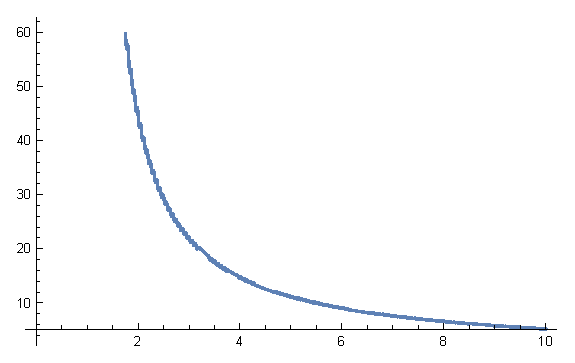
\includegraphics[width=8cm]{nb/trans_amplitude_relative.eps}
  \caption{$U(t)$のグラフ}
  \label{trans_amplitude_fig}
\end{figure}

\subsubsection{追記}

後日分かったように,ここに書いてあることだけじゃ不十分でした.個人的には,複素積分のあたりはよく考え直さないといけないなと思ってます.

\subsection{微細構造定数}

いろいろな意味づけがあるだろうが,シンプルにボーアの原子模型を見ることにする.

\begin{figure}[ht]
  \centering    
  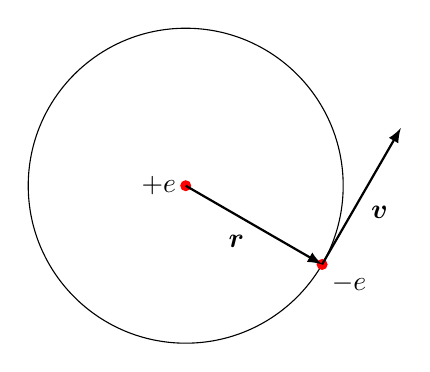
\begin{tikzpicture}[scale=1] 
      \draw [thin] (0,0) circle (2);
      \fill [color=red] ({sqrt(3)},-1) circle (2pt);      
      \fill [color=red] (0,0) circle (2pt);
      \draw (0,0) node [left]{$+e$};
      \draw[-latex,thick] ({sqrt(3)},-1)--({sqrt(3)+1},{-1+1*sqrt(3)});
      \draw[-latex,thick] (0,0)--({sqrt(3)},-1);
      \draw({sqrt(3)/2},-1/2)node [below left]{$\bm{r}$};
      \draw ({sqrt(3)},-1) node [below right]{$-e$};
      \draw ({sqrt(3)+0.5},{-1+0.5*sqrt(3)}) node [below right]{$\bm{v}$};
    \end{tikzpicture}    
    \caption{ボーアの原子模型}
    \label{bohr}
\end{figure}

図\ref{bohr}の運動方程式は
\begin{equation}
  m\frac{v^2}{r}
  =
  \frac{e^2}{4\pi\varepsilon_{0}}\cdot\frac{1}{r^2}
\end{equation}
であり,これに量子条件
\begin{equation}
  mrv
  =
  n\hbar
\end{equation}
を課すと,電子の軌道半径$r_{n}$は$\lambda_{c}=\hbar/mc$とすれば
\begin{equation}
  r_{n}
  =
  \frac{\lambda}{\alpha}n^2
\end{equation}
と書ける.このときの係数
\begin{equation}
  \alpha
  =
  \frac{e^2}{4\pi\varepsilon_{0}\hbar c}
\end{equation}
が\textbf{微細構造定数}である.

\subsection{テンソルカレントの保存量}

ラグランジアン$\mathcal{L}$が微小変位$x^{\mu}\rightarrow x^{\mu}-a^{\mu}$に対して
\begin{equation}
  \mathcal{L}
  \rightarrow
  \mathcal{L}
  +
  a^{\nu}\partial_{\mu}\mathcal{J}^{\mu}_{\ \nu}
\end{equation}
と発散項だけ変化できる.一方で,ラグランジアンの変化は,直接計算すれば
\begin{align}
  a^{\nu}
  \left(  
    \Delta \mathcal{L}
  \right)_{\nu}
  &=
  a^{\nu}\partial_{\mu}
  \left(  
    \pdv{\mathcal{L}}{(\partial_{\mu}\mathcal{L})}\left( \Delta\phi \right)_{\nu}
  \right)
  \nonumber
  \\
  &=
  a^{\nu}\partial_{\mu}
  \left(  
    \pdv{\mathcal{L}}{(\partial_{\mu}\mathcal{L})}\partial_{\nu}\phi
  \right)
\end{align}
なので
\begin{equation}
  j^{\mu}_{\ \nu}(x)
  =
  \pdv{\mathcal{L}}{(\partial_{\mu}\mathcal{L})}\partial_{\nu}\phi
  -
  \mathcal{J}^{\mu}_{\ \nu}
\end{equation}
とすれば
\begin{equation}
  \partial_{\mu}j^{\mu}_{\ \nu}=0
\end{equation}
となる.つまり,これらは$\nu=0,1,2,3$の4つの方程式.

\subsection{規格化}

完全性を
\begin{equation}
  \int\dd^3 \bm{x} \ket{\bm{x}}\bra{\bm{x}}
  =
  1
  \ ,\ \ 
  \int\frac{\dd^3 \bm{p}}{(2\pi)^3} \ket{\bm{p}}\bra{\bm{p}}
  =
  1
\end{equation}
とセッティングした場合に,基底の変換が
\begin{equation}
  \ev*{\bm{x}|\bm{p}}
  =
  e^{i\bm{p}\cdot\bm{x}}
\end{equation}
であることをみる.このときconsistentなのは
\begin{equation}
  \ev*{\bm{x}|\bm{x}'}=\delta^{(3)}(\bm{x}-\bm{x}')
  \ ,\ \ 
  \ev*{\bm{p}|\bm{p}'}=(2\pi)^{3}\delta^{(3)}(\bm{p}-\bm{p}')
\end{equation}
だが\footnote{
  ここでは
  \begin{equation}
    \delta^{(3)}(\bm{x})
    =
    \int\frac{\dd^3 \bm{k}}{(2\pi)^3}
    e^{i\bm{k}\cdot\bm{x}}
    \nonumber
  \end{equation}
  としている.
},それは
\begin{align}
  \ev*{\bm{x}|\bm{x}'}
  &=
  \int\frac{\dd^3 \bm{p}}{(2\pi)^3}\ev*{\bm{x}|\bm{p}}\ev*{\bm{p}|\bm{x}'}
  \nonumber
  \\
  &=
  \int\frac{\dd^3 \bm{p}}{(2\pi)^3}e^{i\bm{p}\cdot(\bm{x}-\bm{x}')}
  \nonumber
  \\
  &=
  \delta^{(3)}(\bm{x}-\bm{x}')
  \\
  \ev*{\bm{p}|\bm{p}'}
  &=
  (2\pi)^3\int\frac{\dd^3}{(2\pi)^3} \bm{x}\ev*{\bm{p}|\bm{x}}\ev*{\bm{x}|\bm{p}'}
  \nonumber
  \\
  &=
  (2\pi)^{3}\delta^{(3)}(\bm{p}-\bm{p}')
  \label{comp}
\end{align}
である.
\\

ここでの話は残念ながらnotationに依存しており,例えば
\begin{equation}
  \int\dd^3 \bm{p}\ketbra{p}{p}=1
\end{equation}
とすると,直交関係
\begin{equation}
  \ev*{\bm{x}|\bm{x}'}=\delta^{(3)}(\bm{x}-\bm{x}')
  \ ,\ \ 
  \ev*{\bm{p}|\bm{p}'}=\delta^{(3)}(\bm{p}-\bm{p}')
  \label{ortho}
\end{equation}
に対して\footnote{
  $p$の完全性と規格化条件の$2\pi$は関係している.例えば,完全性\eqref{comp}のほうが決定したとして,直交条件\eqref{ortho}の係数に$2\pi$をつけると等式が成り立たないことを確認するとよい.簡単な1次元で
  \begin{equation}
    \ev*{p|p'}=2\pi\delta(p-p')
    \tag{??}
  \end{equation}
  だとすると,
  \begin{equation}
    \ev*{p|p'}
    =
    2\pi\ev*{p|p'}
    \tag{!?}
  \end{equation}
  がでてきてまずい.
}
\begin{equation}
  \ev*{\bm{x}|\bm{p}}
  =
  \frac{1}{(2\pi)^{3/2}}e^{i\bm{p}\cdot\bm{x}}
\end{equation}
でconsistent.

\subsection{生成子について}

時間発展や空間並進の生成子\footnote{
  以後,generatorというかもしれない.
}は,$H$や$p$であった.これはなんだったかというと
\begin{equation}
  e^{-iHt}\ket{t_{0}}=\ket{t+t_{0}}
  \ ,\ 
  e^{-ipx}\ket{x_{0}}=\ket{x+x_{0}}
\end{equation}
というような関係があることを意味していた.時間発展はシュレーディンガー方程式
\begin{equation}
  i\partial_{0}\ket{t}
  =
  H\ket{t}
  \label{t_ev}
\end{equation}
から,空間並進は
\begin{equation}
  xe^{-ipx}\ket{x_{0}}
  =
  (x+x_{0})(e^{-ipx}\ket{x_{0}})
\end{equation}
からくる\footnote{
  計算過程はこう.$e^{-ipx}$を展開してから交換関係を使うと,
  \begin{equation}
    \hat{x}\sum_{n=0}^{\infty}\frac{(-ix)^n}{n!}\hat{p}^{n}
    =
    \sum_{n=0}^{\infty}\frac{(-ix)^n}{n!}\hat{p}^{n}\hat{x}
    +
    x\sum_{n=0}^{\infty}\frac{(-ix)^n}{n!}\hat{p}^{n}
    \nonumber
  \end{equation}
  だから.
}.両者の共通点は,式\eqref{t_ev}と$p$の表示を並べてみるとわかりやすくて
\begin{align}
  H\ket{\psi}
  &=
  i\partial_{0}\ket{\psi}
  \\
  p\ket{\psi}
  &=
  -i\partial_{1}\ket{\psi}
\end{align}
ということ\footnote{
  だから,$p^{\mu}=i\partial^{\mu}$とおく.
}.
\\

さて,生成子が何かといわれれば,解析力学的にいうと,ある正準変換の無限小変換を生成する$S$のことをいう.この変換である物理量$F$が変換されるとき
\begin{equation}
  \dd F
  =
  \{ F,S \}_{\text{P}}
\end{equation}
という関係式が成り立つ.これを量子論に移行すればよい.例えばテキストでは,
\begin{equation}
  Q
  =
  \int j^{0}(\bm{x}) \dd^3 \bm{x}
\end{equation}
がgeneratorになっているはずで,
\begin{align}
  [\phi,Q]
  &=
  \int \dd^3 \bm{x}^{\prime}\ [\phi(x),j^{0}(x^{\prime})]
  \nonumber
  \\
  &=
  \int \dd^3 \bm{x}^{\prime}\ 
  \left[  
    \phi(x),\pdv{\mathcal{L}}{\dot{\phi}}\Delta\phi-\mathcal{J}^{0}
  \right]
  \nonumber
  \\
  &=
  \int \dd^3 \bm{x}^{\prime}\ [ \phi(x),\pi(x') ]\Delta\phi
  \nonumber
  \\
  &=\Delta\phi
\end{align}
でOK.

\subsection{ローレンツ変換後の状態の一意性}

ローレンツ変換
\begin{equation}
  \left\{
    \begin{alignedat}{1}
      E^{\prime}
      &=  
      \gamma(E+\beta p_{3})
      \\
      p_{3}^{\prime}
      &=
      \gamma(\beta E+p_{3})      
    \end{alignedat}
  \right.
\end{equation}
をしたときに,$\vec{p}=\vec{q}$の条件も変換されて$\vec{p}^{\prime}=\vec{q}^{\prime}$となるが,これを満たす状態は1つのみか,という話.$p_{1},p_{2}$は不変なので$p_{3}$だけ考えればいい.第3成分は
\begin{equation}
  \beta E_{\vec{p}}+p_{3}
  =
  \beta E_{\vec{q}}+q_{3}
\end{equation}
となるが,これを満たす$p,q$は1つか.$E$をexplicitに書くと
\begin{equation}
  \beta \sqrt{p_{1}^{2}+p_{2}^{2}+p_{3}^{2}+m^2}+p_{3}
  =
  \beta \sqrt{p_{1}^{2}+p_{2}^{2}+q_{3}^{2}+m^2}+q_{3}
  \label{eq51}
\end{equation}
となる\footnote{
  $\vec{p},\vec{q}$の1,2成分は一致している.
}.関数
\begin{equation}
  f(x)
  =
  \beta\sqrt{x^2+p_{1}^{2}+p_{2}^{2}+m^2}+x
\end{equation}
を考えれば,これは単調増加関数なので単射\footnote{
  この関数は,$x$が負でもちゃんと単射です.なぜなら
  \begin{equation}
    f^{\prime}(x)
    =
    \frac{\beta x}{\sqrt{x^2+p_{1}^{2}+p_{2}^{2}+m^2}}
    +
    1
    \nonumber
  \end{equation}
  ですが,
  \begin{equation}
    \left|
      \frac{\beta x}{\sqrt{x^2+p_{1}^{2}+p_{2}^{2}+m^2}}
    \right|
    =
    |\beta|
    \cdot
    \frac{1}{\sqrt{1+(p_{1}^{2}+p_{2}^{2}+m^2)/x^2}}
    <
    1
    \nonumber
  \end{equation}
  だからです.
}.よって,\eqref{eq51}を満たす$p_{3},q_{3}$の組は1つのみ.

ちなみに,$E^{\prime}$の式は
  \begin{align}
    {E^{\prime}}^{2}
    &=
    |\vec{p}^{\prime}|^2+m^2
    \nonumber
    \\
    &=
    p_{1}^2
    +
    p_{2}^2
    +
    \gamma^2 (\beta E+p_{3})^2
    +
    m^2
    \nonumber
    \\
    &=
    |\vec{p}|^2
    +
    m^2
    +
    \gamma^2 \beta^2 E^2
    +
    2\gamma^2 \beta E p_{3}
    +
    (\gamma^2-1)p_{3}^2
    \nonumber
    \\
    &=
    (1+\gamma^2\beta^2)E^2
    +
    2\gamma^2 \beta E p_{3}
    +
    \gamma^2 \beta^2 p_{3}^2
    \nonumber
    \\
    &=
    \gamma^2
    (E+\beta p_{3})^2
  \end{align}
となるので\footnote{
  ここで,
  \begin{equation}
    \gamma^2-1
    =
    \gamma^2 \beta^2
    \ ,\ 
    1+\gamma^2 \beta^2
    =
    \gamma^2
    \nonumber
  \end{equation}
  などを用いている.
},この式は$p_{3}^{\prime}=\gamma(\beta E+p_{3})$が成り立っていれば,自動に成立する式である.

\subsection{式(2.52)のブランチカットの話}
積分
\begin{equation}
  I
  \coloneqq
  \int_{-\infty}^{\infty}
  \dd p\ 
  \frac{pe^{ipr}}{\sqrt{p^2+m^2}}
\end{equation}
の評価を考える\footnote{
  ちなみに,今回はこの記事\cite{contour}やこの記事\cite{branch}のExm.10.4.2を参考にしています.
}.この積分は経路は図\ref{cont_a}である\footnote{
  ただし,$+im$と$-im$から出ているジグザグな線は$\sqrt{p^2+m^2}$のブランチカット.
}.

\begin{figure}[ht]
  \centering
  \begin{tikzpicture}[scale=1.4]
    \draw[ultra thick](-2,0) -- (2,0);
    \draw[-{Latex[length=2.5mm]}](-0.1,0)--(0,0);
    \draw[decorate, decoration={zigzag, segment length=6, amplitude=2}] (0,0.5) -- (0,2);    
    \draw[decorate, decoration={zigzag, segment length=6, amplitude=2}] (0,-0.5) -- (0,-2);
    \fill (0,0.5) circle (2pt) node [right]{$+im$};    
    \fill (0,-0.5) circle (2pt) node [left]{$-im$};  
  \end{tikzpicture}
  \caption{変更前の経路}
  \label{cont_a}
\end{figure}

被積分関数を
\begin{equation}
  f(p)
  \coloneqq  
  \frac{pe^{ipr}}{\sqrt{p^2+m^2}}
\end{equation}
とすれば,(多分)ブランチカット以外では正則なので,経路をひん曲げることができて,積分$I$は
\begin{equation}
  I
  =
  \int_{C_{1}}f
  +
  \int_{C_{2}}f
  +
  \int_{C}f
\end{equation}
と分割できる.

\begin{figure}[ht]
  \centering
  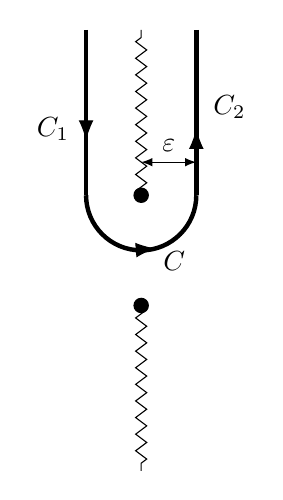
\begin{tikzpicture}[scale=1.4]
    \draw[decorate, decoration={zigzag, segment length=6, amplitude=2}] (0,0.5) -- (0,2);    
    \draw[decorate, decoration={zigzag, segment length=6, amplitude=2}] (0,-0.5) -- (0,-2);
    \fill (0,0.5) circle (2pt);    
    \fill (0,-0.5) circle (2pt);
    \draw[ultra thick] (-0.5,2) -- (-0.5,0.5);
    \draw[ultra thick] (0.5,2) -- (0.5,0.5);
    \draw[-{Latex[length=2.5mm]}](-0.5,1.1)--(-0.5,1.0);
    \draw[-{Latex[length=2.5mm]}](0.5,1.0)--(0.5,1.1);    
    \draw[ultra thick] (-0.5,0.5) arc (180:360:0.5);        
    \draw[-{Latex[length=2.5mm]}] (-0.5,0.5) arc (180:285:0.5);
    \draw (0.3,-0.1) node {$C$};     
    \draw (0.8,1.3) node {$C_{2}$};      
    \draw (-0.8,1.1) node {$C_{1}$}; 
    \draw [latex-latex] (0,0.8) -- (0.5,0.8);
    \draw (0.25,0.95) node []{$\varepsilon$};
  \end{tikzpicture}
  \caption{変更後の経路}
  \label{cont2}
\end{figure}

円$C$の半径を小さくすれば,その経路の積分の寄与が小さくなるので,その部分は無視できる.よって,$C_{1},C_{2}$を考えればよい.$C_{1}$の微分を計算してみると,$p=i\rho-\varepsilon$より
\begin{align}
  \int_{C_{1}}f
  &=
  \int_{i\infty}^{im}
  \dd p
  \frac{pe^{ipr}}{\sqrt{p^2+m^2}}
  \nonumber
  \\
  &=  
  \int_{\infty}^{m}
  \dd i\rho
  \frac{i\rho e^{-\rho r}}{\sqrt{(i\rho-\varepsilon)^2+m^2}}
  \nonumber
  \\
  &=
  \frac{1}{i}
  \int_{m}^{\infty}
  \dd \rho
  \frac{\rho e^{-\rho r}}{\sqrt{\rho^2-m^2+2i\rho \varepsilon}}
  \label{f_c1}
\end{align}
である.ここで,点$\rho^2-m^2-2i\rho\varepsilon$の偏角を考えてみると,図\ref{p1}より$\arg(\rho^2-m^2+2i\rho\varepsilon)\rightarrow 0$に収束する.したがって,
\begin{equation}
  \sqrt{\rho^2-m^2+2i\rho \varepsilon}
  =
  \sqrt{\rho^2-m^2}
\end{equation}
と評価できるので
\begin{equation}
  \int_{C_1}f
  =
  \frac{1}{i}\int_{m}^{\infty}
  \dd \rho
  \frac{\rho e^{-\rho r}}{\sqrt{\rho^2-m^2}}
\end{equation}
となる.

\begin{figure}
  \centering
  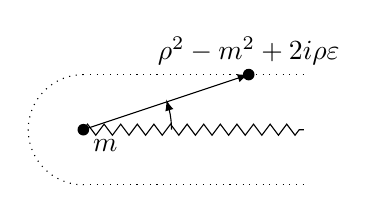
\begin{tikzpicture}[scale=1.4]
    \draw[decorate, decoration={zigzag, segment length=6, amplitude=2}] (0,0) -- (2,0);
    \draw[dotted] (0,0.5) -- (2,0.5);    
    \draw[dotted] (0,-0.5) -- (2,-0.5);
    \draw[dotted] (0,0.5) arc (90:270:0.5);
    \fill (0,0) circle (1.5pt) node [below right]{$m$};
    \draw[-latex](0,0) -- (1.5,0.5);
    \fill (1.5,0.5) circle(1.5pt) node [above]{$\rho^2-m^2+2i\rho\varepsilon$};
    \draw[-latex] (0.8,0) arc (0:20:0.8);
  \end{tikzpicture}
  \caption{$p=i\rho-\varepsilon$のとき}
  \label{p1}
\end{figure}

さて,$C_{2}$を評価しよう.積分は
\begin{equation}
  \int_{C_{2}}f
  =
  -\frac{1}{i}\int_{m}^{\infty}
  \dd \rho
  \frac{\rho e^{-\rho r}}{\sqrt{\rho^2-m^2-2i\rho\varepsilon}}
\end{equation}
であり,図\ref{p2}より$\arg(\rho^2-m^2+2i\rho\varepsilon)\sim 2\pi$なので,$\sqrt{\rho^2-m^2-2i\rho\varepsilon}\sim-\sqrt{\rho^2-m^2}$となり
\begin{equation}
  \int_{C_{2}}f
  =
  \frac{1}{i}\int_{m}^{\infty}
  \dd \rho
  \frac{\rho e^{-\rho r}}{\sqrt{\rho^2-m^2}}
\end{equation}
である\footnote{
  普通,$C_{1}$と$C_{2}$は逆向きなので打ち消しそうだが,同じリーマン面で積分するので$\sqrt{p^2+m^2}$の符号が異なるため,重なって$0$にならない.
}.

\begin{figure}
  \centering
  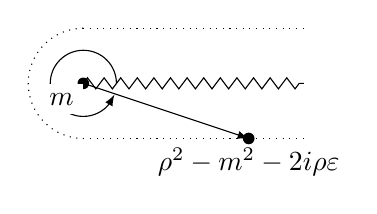
\begin{tikzpicture}[scale=1.4]
    \draw[decorate, decoration={zigzag, segment length=6, amplitude=2}] (0,0) -- (2,0);
    \draw[dotted] (0,0.5) -- (2,0.5);    
    \draw[dotted] (0,-0.5) -- (2,-0.5);
    \draw[dotted] (0,0.5) arc (90:270:0.5);
    \draw[-latex](0,0) -- (1.5,-0.5);
    \fill (1.5,-0.5) circle(1.5pt) node [below]{$\rho^2-m^2-2i\rho\varepsilon$};
    \draw[-latex] (0.3,0) arc (0:340:0.3);
    \fill (0,0) circle (1.5pt) node [below left,fill=white]{$m$};
  \end{tikzpicture}
  \caption{$p=i\rho+\varepsilon$のとき}
  \label{p2}
\end{figure}

したがって
\begin{equation}
  I
  =
  \int_{C_{1}}f
  +
  \int_{C_{2}}f
  =
  \frac{2}{i}\int_{m}^{\infty}
  \dd \rho
  \frac{\rho e^{-\rho r}}{\sqrt{\rho^2-m^2}}
\end{equation}
となり,
\begin{equation}
  D(x-y)
  =
  -\frac{1}{4\pi^2 r}
  \int_{m}^{\infty}
  \dd \rho
  \frac{\rho e^{-\rho r}}{\sqrt{\rho^2-m^2}}
  \label{prop}
\end{equation}
となる\footnote{
  符号については\ref{ps2}を.
}.

ちなみに,簡単な解釈は,リーマン球面を考えてやればこの積分は$p=\infty$という点でブランチをまたぐ,という意味で解釈するのが楽でしょう.ただ,具体的な値は出てきませんが.発想はコーシーの積分定理と同じです.

\subsubsection{追記 I}
そういえば,積分路の変更は,コーシーの定理から来ているが,その際,外側の積分が上半円で$0$にconvergeすることは言ってやらないといけない.$p=Re^{i\theta}$とすれば
\begin{equation}
  \int_{C}f
  =
  \int_{0}^{\pi}
  Re^{i\theta}\dd \theta
  \frac{Re^{i\theta}e^{iRe^{i\theta}pr}}{\sqrt{R^2e^{2i\theta}+m^2}} 
\end{equation}
である.ただし,$0\leq\theta\leq\pi$である.絶対値をとってやれば
\begin{align}
  \left|
    \int_{0}^{\pi}
  Re^{i\theta}\dd \theta
  \frac{Re^{i\theta}e^{iRe^{i\theta}pr}}{\sqrt{R^2e^{2i\theta}+m^2}} 
  \right|
  &\leq
  R^2
  \int_{0}^{\pi}
  \dd \theta
  \left|    
  \frac{e^{-Rpr\sin\theta}}{\sqrt{R^2e^{2i\theta}+m^2}} 
  \right|
  \nonumber
  \\
  &\rightarrow
  0
  \ \ \ 
  (R\rightarrow \infty)
\end{align}
である\footnote{
  まあ,なんか前に私が詰められた感じで,もっと細かく詰められるかもしれませんが,そもそもこの積分が収束するかどうかわからないのにここら辺を厳密にやろうとするのはナンセンスかとおもうので,こんな感じでいいんじゃないでしょうか.
}\footnote{さらに追記.この積分,$0$に収束しない!けど,「教科書もそれには目をつむってひとまず進んでいる」というのが先生の意見.}.

\subsubsection{追記 II}
\label{ps2}
どうやら\eqref{f_c1}で$-\rho^2+m^2-2i\pi\varepsilon$の偏角をちゃんと吟味しなかったため,\eqref{prop}の符号が教科書とずれてしまった模様.

\subsection{デルタ関数の性質・コーシーの主値*}

次の公式
\begin{equation}
  \frac{1}{x+i\varepsilon}
  =
  P\left( \frac{1}{x} \right)
  -
  i\pi\delta(x)
\end{equation}
について解説する\footnote{
  こういうのは知っておいたほうがいいそうです.
}.




\subsection{ディラック代数から構成される生成子の交換関係}

$\gamma$行列で定義される次の量
\begin{equation}
  S^{\mu\nu}
  \coloneqq
  \frac{i}{4}[\gamma^{\mu},\gamma^{\nu}]
\end{equation}
がgeneratorであること,すなわち,次の交換関係
\begin{equation}
  [S^{\mu\nu},S^{\rho\sigma}]
  =
  i(
    g^{\nu\rho}S^{\mu\sigma}
    -
    g^{\mu\rho}S^{\nu\sigma}
    -
    g^{\nu\sigma}S^{\mu\rho}
    +
    g^{\mu\sigma}S^{\nu\rho}
  )
  \label{comu}
\end{equation}
を満たすことを確認しておく.なお,$\gamma$行列の定義は
\begin{equation}
  \{
    \gamma^{\mu},\gamma^{\nu}
  \}
  =
  2g^{\mu\nu}
\end{equation}
である.さて,\eqref{comu}の左辺を展開してみると
\begin{align}
  [S^{\mu\nu},S^{\rho\sigma}]
  &=
  \left( \frac{i}{4} \right)^{2}
  [
    \gamma^{\mu}\gamma^{\nu}-\gamma^{\nu}\gamma^{\mu}
    ,
    \gamma^{\rho}\gamma^{\sigma}-\gamma^{\sigma}\gamma^{\rho}
  ]
  \nonumber
  \\
  &=
  \left( \frac{i}{4} \right)^{2} \cdot 4
  [
    g^{\mu\nu}-\gamma^{\nu}\gamma^{\mu}
    ,
    g^{\rho\sigma}-\gamma^{\sigma}\gamma^{\rho}
  ]
  \nonumber
  \\
  &=
  \left( \frac{i}{4} \right)^{2} \cdot 4
  [
    \gamma^{\nu}\gamma^{\mu}
    ,
    \gamma^{\sigma}\gamma^{\rho}
  ]
  \label{foo}
\end{align}
となる\footnote{
  ここで
  $$
  \gamma^{\mu}\gamma^{\nu}-\gamma^{\nu}\gamma^{\mu}
  =
  \{\gamma^{\mu},\gamma^{\nu}\}-2\gamma^{\nu}\gamma^{\mu}
  =
  2(g^{\mu\nu}-\gamma^{\nu}\gamma^{\mu})
  $$
  の関係を用いて計算している.
}.ここで,$[
  \gamma^{\nu}\gamma^{\mu}
  ,
  \gamma^{\sigma}g^{\rho}
]$を計算すると
\begin{align}
  [
  \gamma^{\nu}\gamma^{\mu}
  ,
  \gamma^{\sigma}\gamma^{\rho}
  ]
  &=
  \gamma^{\nu}\gamma^{\sigma}
  [
  \gamma^{\mu}
  ,
  \gamma^{\rho}
  ]
  +
  \gamma^{\nu}
  [
  \gamma^{\mu}
  ,
  \gamma^{\sigma}
  ]
  \gamma^{\rho}
  +
  \gamma^{\sigma}
  [
  \gamma^{\nu}
  ,
  \gamma^{\rho}
  ]
  \gamma^{\mu}
  +
  [
  \gamma^{\nu}
  ,
  \gamma^{\sigma}
  ]
  \gamma^{\rho}\gamma^{\mu}
  \nonumber
  \\
  &=
  \uline{
    \gam{\nu}{\sigma}{\mu}{\rho}
  }
  -
  \dashuline{
    \gam{\nu}{\sigma}{\rho}{\mu}
  }
  +
  \gam{\nu}{\mu}{\sigma}{\rho}
  -
  \uline{
    \gam{\nu}{\sigma}{\mu}{\rho}
  }
  \nonumber
  \\
  &\quad
  +
  \uwave{
    \gam{\sigma}{\nu}{\rho}{\mu}
  }
  -
  \gam{\sigma}{\rho}{\nu}{\mu}
  +
  \dashuline{
    \gam{\nu}{\sigma}{\rho}{\mu}
  }
  -
  \uwave{
    \gam{\sigma}{\nu}{\rho}{\mu}
  }
  \nonumber
  \\
  &=
  \gam{\nu}{\mu}{\sigma}{\rho}
  -
  \gam{\sigma}{\rho}{\nu}{\mu}
  \label{rarara}
\end{align}
となる.ここで,第1項が第2項と打ち消しあうように,$\gam{\nu}{\mu}{\sigma}{\rho}$のうちの$\gamma^{\sigma}\gamma^{\rho}$を,先頭にもってくる作業をする.交換関係に気をつければ
\begin{align}
  \gam{\nu}{\mu}{\sigma}{\rho}
  &=
  \gamma^{\nu}
  (
    2g^{\mu\sigma}
    -
    \gamma^{\sigma}\gamma^{\mu}
  )
  \gamma^{\rho}
  \nonumber
  \\
  &=
  2g^{\mu\sigma}\gamma^{\nu}\gamma^{\rho}
  -
  \gam{\nu}{\sigma}{\mu}{\rho}
  \nonumber
  \\
  &=
  2g^{\mu\sigma}\gamma^{\nu}\gamma^{\rho}
  -
  (2g^{\nu\sigma}-\gamma^{\sigma}\gamma^{\nu})
  \gamma^{\mu}\gamma^{\rho}
  \nonumber
  \\
  &=
  2g^{\mu\sigma}\gamma^{\nu}\gamma^{\rho}
  -
  2g^{\nu\sigma}\gamma^{\mu}\gamma^{\rho}
  +
  \gam{\sigma}{\nu}{\mu}{\rho}
  \nonumber
  \\
  &=
  2g^{\mu\sigma}\gamma^{\nu}\gamma^{\rho}
  -
  2g^{\nu\sigma}\gamma^{\mu}\gamma^{\rho}
  +
  \gamma^{\sigma}\gamma^{\nu}
  (
    2g^{\mu\rho}-\gamma^{\rho}\gamma^{\mu}
  )
  \nonumber
  \\
  &=
  2g^{\mu\sigma}\gamma^{\nu}\gamma^{\rho}
  -
  2g^{\nu\sigma}\gamma^{\mu}\gamma^{\rho}
  +
  2g^{\mu\rho}\gamma^{\sigma}\gamma^{\nu}
  -
  \gam{\sigma}{\nu}{\rho}{\mu}
  \nonumber
  \\
  &=
  2g^{\mu\sigma}\gamma^{\nu}\gamma^{\rho}
  -
  2g^{\nu\sigma}\gamma^{\mu}\gamma^{\rho}
  +
  2g^{\mu\rho}\gamma^{\sigma}\gamma^{\nu}
  -
  \gamma^{\sigma}
  (2g^{\nu\rho}-\gamma^{\rho}\gamma^{\nu})
  \gamma^{\mu}
  \nonumber
  \\
  &=
  2g^{\mu\sigma}\gamma^{\nu}\gamma^{\rho}
  -
  2g^{\nu\sigma}\gamma^{\mu}\gamma^{\rho}
  +
  2g^{\mu\rho}\gamma^{\sigma}\gamma^{\nu}
  -
  2g^{\nu\rho}\gamma^{\sigma}\gamma^{\mu}
  +
  \gam{\sigma}{\rho}{\nu}{\mu}
\end{align}
となるので,\eqref{rarara}から
\begin{equation}
  [
  \gamma^{\nu}\gamma^{\mu}
  ,
  \gamma^{\sigma}\gamma^{\rho}
  ]
  =
  2g^{\mu\sigma}\gamma^{\nu}\gamma^{\rho}
  -
  2g^{\nu\sigma}\gamma^{\mu}\gamma^{\rho}
  +
  2g^{\mu\rho}\gamma^{\sigma}\gamma^{\nu}
  -
  2g^{\nu\rho}\gamma^{\sigma}\gamma^{\mu}
\end{equation}
となる.さらにここで,
\begin{equation}
  2\gamma^{\mu}\gamma^{\nu}
  =
  [\gamma^{\mu},\gamma^{\nu}]
  +
  \{\gamma^{\mu},\gamma^{\nu}\}
  =
  [\gamma^{\mu},\gamma^{\nu}]
  +
  2g^{\mu\nu}
\end{equation}
が一般に成立することに注意すれば,
\begin{align}
  [
  \gamma^{\nu}\gamma^{\mu}
  ,
  \gamma^{\sigma}\gamma^{\rho}
  ]
  &=
  g^{\mu\sigma}(\gcomu{\nu}{\rho})
  -
  g^{\nu\sigma}(\gcomu{\mu}{\rho})
  \nonumber
  \\
  &\qquad
  +
  g^{\mu\rho}(\gcomu{\sigma}{\nu})
  -
  g^{\nu\rho}(\gcomu{\sigma}{\mu})
  \nonumber
  \\
  &=
  g^{\mu\sigma}[\gamma^{\nu},\gamma^{\sigma}]
  -
  g^{\nu\sigma}[\gamma^{\mu},\gamma^{\rho}]
  +
  g^{\mu\rho}[\gamma^{\sigma},\gamma^{\nu}]
  -
  g^{\nu\rho}[\gamma^{\sigma},\gamma^{\mu}]
\end{align}
となる.よって,(\ref{foo})に戻ると
\begin{align}
  [S^{\mu\nu},S^{\rho\sigma}]
  &=
  i\cdot
  \frac{i}{4}
  \left[  
    g^{\mu\sigma}[\gamma^{\nu},\gamma^{\sigma}]
    -
    g^{\nu\sigma}[\gamma^{\mu},\gamma^{\rho}]
    +
    g^{\mu\rho}[\gamma^{\sigma},\gamma^{\nu}]
    -
    g^{\nu\rho}[\gamma^{\sigma},\gamma^{\mu}]
  \right]
  \nonumber
  \\
  &=
  i
  ( 
    g^{\mu\sigma}S^{\nu\sigma}
    -
    g^{\nu\sigma}S^{\mu\rho}
    +
    g^{\mu\rho}S^{\sigma\nu}
    -
    g^{\nu\rho}S^{\sigma\mu}
  )
  \nonumber
  \\
  &=
  i(
    g^{\nu\rho}S^{\mu\sigma}
    -
    g^{\mu\rho}S^{\nu\sigma}
    -
    g^{\nu\sigma}S^{\mu\rho}
    +
    g^{\mu\sigma}S^{\nu\rho}
  )
\end{align}
であり,確かに\eqref{comu}を満たしている.








\clearpage

\begin{thebibliography}{99}
  \bibitem{peskin} Peskin, M.E., Schroeder, D.V., 1995. \textit{An Introduction to Quantum Field Theory}. Addison-Wesley Pub. Co, Reading, Mass.
  \bibitem{contour} “Answer to ‘Contour Integrals Around a Branch Cut’,” Dec. 02, 2014. \url{https://math.stackexchange.com/a/1047898} (accessed May 05, 2023).
  \bibitem{branch} “10.4: Integrands with branch cuts,” Sep. 05, 2017. \url{https://math.libretexts.org/Bookshelves/Analysis/Complex_Variables_with_Applications_(Orloff)/10\%3A_Definite_Integrals_Using_the_Residue_Theorem/10.04\%3A_Integrands_with_branch_cuts} (accessed May 05, 2023).
\end{thebibliography}

\end{document}
